\newpage
\section{Дробно-линейные функции, их геометрические свойства: круговое свойство и сохранение симметричности.}


\textbf{Дробно-линейные отображения} --- это функции вида: $$w=\frac{az+b}{cz+d}, \text{где } \ \begin{vmatrix}
    a&b\\
    c&d
\end{vmatrix} \neq 0, \ a,b,c,d\in \mathbb{C}$$

Доопределим функцию выше следующим образом:$$z=-\frac{d}{c}: \ w(-\frac{d}{c}) = \infty$$
$$z = \infty: \ w(\infty) = \left[\begin{gathered}\frac{a}{c}, \ c\neq 0\\
\infty, \ c=0
\end{gathered}
\right.$$
Тогда ДЛО: $w: \overline{\mathbb{C}}\to \overline{\mathbb{C}}$


\textbf{Круговое свойство ДЛО}\\
Любое ДЛО преобразует обобщенную окружность (окружность и ли прямая в $\overline{\mathbb{C}}$) в обобщенную окружность.

\begin{proof}
    \ \\
    1) случай, когда $c=0$:\\
    $L: \ w = az+b$\\
    $z \overset{L_1}{\rightarrow} z_1=az \overset{L_2}{\rightarrow}z_2=z_1+b$\\
    $L_1$ --- растяжение с поворотом: окружность перейдет в окружность, а прямая в прямую\\
    $L_2$ --- сдвиг: окружность перейдет в окружность, а прямая в прямую\\[2mm]
    2) случай, когда $c\neq 0$:\\
    $L: \ w=\frac{az+b}{cz+d}=\frac{a}{c} +\left(\frac{az+b}{cz+d}-\frac{a}{c}\right) = \frac{a}{c}+\frac{caz+bz-acz-ad}{c(cz+d)}=$\\[2mm]
    $\frac{a}{c}+\frac{bc-ad}{c(cz+d)}=\frac{a}{c}+\frac{\frac{bc-ad}{c}}{z+\frac{d}{c}}$\\[2mm]
    Обозначим $A=\frac{a}{c}, \ B=\frac{bc-ad}{c}, \ C=\frac{d}{c}:$\\[2mm]
    $L: \ w = A + \frac{B}{z+C}$\\[2mm]
    $z \overset{L_1}{\rightarrow} z_1=z+C \overset{L_2}{\rightarrow}z_2=\frac{1}{z_1} \overset{L_3}{\rightarrow}z_3=B\cdot z_2 \overset{L_4}{\rightarrow} w = A+z_3$\\[2mm]
    Отображения $L_1$ и $L_4$ --- сдвиги, $L_3$ --- растяжение с поворотом. Они переводят окружности в окружности, а прямые в прямые.\\
    Рассмотрим отображение $L_2: \ w=\frac{1}{z}$\\[2mm] 
    Общее уравнение обобщённой окружности на плоскости $xOy$:
    $$E(x^2+y^2) +F_1x + F_2 y + G=0$$
    $$E, F_1, F_2, G \in \mathbb{R}, \ (E, F_1, F_2, G) \neq (0, 0, 0, 0)$$
    Запишем это уравнение через переменную $z=x+iy$:
    $$x=\frac{z+\overline{z}}{2}, \ y=\frac{z-\overline{z}}{2i}=i\frac{\overline{z}-z}{2}$$
    $$Ez\overline{z}+F_1\frac{z+\overline{z}}{2}+F_2i\frac{\overline{z}-z}{2}+G=0$$
    $$Ez\overline{z}+Fz+\overline{F}\overline{z}+G=0,$$
    $$\text{где }F=\frac{1}{2}F_1-\frac{1}{2}iF_2 \in \mathbb{C}, \ \overline{F} = \frac{1}{2}F+\frac{1}{2}iF_2$$
    Тогда кривая, полученная в результате преобразования $L_2$ задается уравнением:
    $$E\frac{1}{z}\overline{\left(\frac{1}{z}\right)}+F\frac{1}{z}+\overline{F}\overline{\left(\frac{1}{z}\right)}+G=0|\cdot z\overline{z}$$
    $$E+F\overline{z}+\overline{F}z+Gz\overline{z}=0,$$
    что является уравнением обобщенной окружности.
    Значит отображение $L_2$ переводит обобщенную окружность в обобщенную окружность.
\end{proof}


\textbf{Свойство ДЛО сохранения симметричности}\\
Произвольное ДЛО $L$ преобразует любые точки $z$ и $z^*$, симметричные относительно обобщенной окружности $\Gamma$, в точки $L(z)$ и $L(z^*)$, симметричные относительно обобщенной окружности $L(\Gamma)$.

\begin{figure}[!ht]
    \begin{center}
    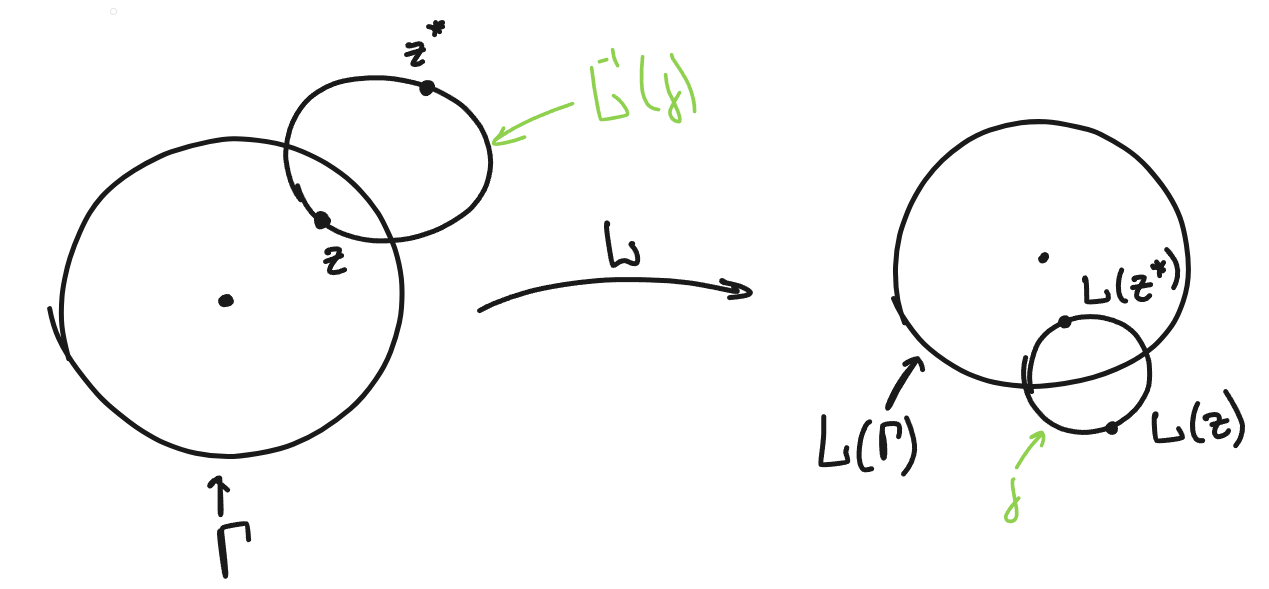
\includegraphics[scale=0.4]{answers/img/ans8.png}
    \label{pic08}
    \end{center}
\end{figure}

\begin{proof}
    \ \\
    Пусть $\gamma$ --- произвольная обобщенная окружность, проходящая через точки $L(z)$ и $L(z^*)$. Тогда $L^{-1}(\gamma)$ --- обобщенная окружность по круговому свойству ДЛО.\\[2mm]
    Так как $L(z)$, $L(z^*) \in \gamma$, то:\\
    $L^{-1}(L(z))=z \in L^{-1}(\gamma)$ и $L^{-1}(L(z^*))=z^*\in L^{-1}(\gamma)$.\\[2mm]
    По определению симметричных точек окружности $\Gamma$ и $L^{-1}(\gamma)$ ортогональны. ДЛО $L$ сохраняет углы, а значит $L(\Gamma)$ ортогональна $L(\gamma)$. 
\end{proof}
